\begin{example}[Définition 10 : $a > b$ : $a = 7$, $b = 3$]
    ~
    \begin{itemize}
        \item Limites pour toute séquence de $\mathcal{PF}_{7,3}$
            une fois triée : $[1,\ 1 \frac{3}{7},\ 1 \frac{6}{7},\ 
            2 \frac{2}{7},\ 2 \frac{5}{7},\ 3 \frac{1}{7},\ 
            3 \frac{4}{7}]$
        \item $f_1 = (2, 1, 1, 3, 2, 3, 1) \in
            \mathcal{PF}_{7,3}$
        \item $f_2 = (2, 1, 2, 3, 2, 3, 1) \notin
            \mathcal{PF}_{7,3}$, bien que $f_2 \in
            \mathcal{PF}_7$
    \end{itemize}
\end{example}

\begin{example}[Définition 10 : $a < b$ : $a = 5$, $b = 7$]
    ~
    \begin{itemize}
        \item Limites pour toute séquence de $\mathcal{PF}_{5,7}$
            une fois triée : $[1,\ 2 \frac{2}{5},\ 3 \frac{4}{5},\ 
            5 \frac{1}{5},\ 6 \frac{3}{5}]$
        \item $f_3 = (6, 3, 5, 1, 2) \in
            \mathcal{PF}_{5,7}$, bien que $f_3 \notin
            \mathcal{PF}_5$
        \item $f_4 = (6, 3, 5, 1, 3) \notin
            \mathcal{PF}_{5,7}$\\
    \end{itemize}
\end{example}

\begin{example}[Théorème 6 : $a = 3, b = 5$]
    ~\\
    \begin{itemize*}\\
        \item $pf_{a,b} = 25$
        \item Limites : $[1,\ 2 \frac{2}{3},\ 
            4 \frac{1}{3}]$\\\\
        \subitem $(1, 1, 1)$
        \subitem $(1, 1, 2)$
        \subitem $(1, 1, 3)$
        \subitem $(1, 1, 4)$
        \subitem $(1, 2, 1)$
        \subitem $(1, 2, 2)$
        \subitem $(1, 2, 3)$
        \subitem $(1, 2, 4)$
        \subitem $(1, 3, 1)$
        \subitem $(1, 3, 2)$
        \subitem $(1, 4, 1)$
        \subitem $(1, 4, 2)$
        \subitem $(2, 1, 1)$
        \subitem $(2, 1, 2)$
        \subitem $(2, 1, 3)$
        \subitem $(2, 1, 4)$
        \subitem $(2, 2, 1)$
        \subitem $(2, 3, 1)$
        \subitem $(2, 4, 1)$
        \subitem $(3, 1, 1)$
        \subitem $(3, 1, 2)$
        \subitem $(3, 2, 1)$
        \subitem $(4, 1, 1)$
        \subitem $(4, 1, 2)$
        \subitem $(4, 2, 1)$\\
    \end{itemize*}
\end{example}

\begin{example}[Définition 11 : $a > b : a = 7, b = 3$]
    ~\\
    \begin{align*}
        &w_1 = 1110011110 \text{ n'est \emph{pas} un 7, 3 - mot de
        Dyck, car } |11100|_1 = 3\\
        & \hspace{5cm} < \frac{7}{3}|11100|_0
        = \frac{14}{3} = 4 \frac{1}{3}.\\
        &w_2 = 1110111010 \text{ \emph{est} un 7, 3 - mot de Dyck : }\\
    \end{align*}
    \input{fig/fig12.tex}
\end{example}

\begin{example}[Définition 11 : $a < b : a = 3, b = 5$]
    ~\\
    \begin{align*}
        &w_1 = 10100010 \text{ n'est \emph{pas} un 3, 5 - mot de
        Dyck, car } |101000|_1 = 2\\
        & \hspace{5cm} < \frac{3}{5}|101000|_0
        = \frac{12}{5} = 2 \frac{2}{5}.\\
        &w_2 = 10100100 \text{ \emph{est} un 3, 5 - mot de Dyck : }\\
    \end{align*}
    \begin{center}
    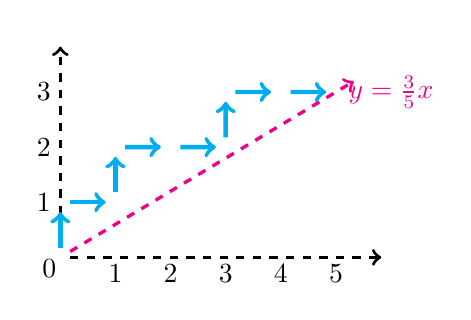
\begin{tikzpicture}[scale=0.7]
        \node (a) at (0, 0) {};
        \node (b) at (0, 4) {};
        \node (c) at (6, 0) {};
        \node (d) at (5.5, 3.3) {};
        \node (e) at (6, 3) [color = magenta]
            {$y = \frac{3}{5}x$}; 
        \draw [dashed, very thick, ->] (a) to (b);
        \draw [dashed, very thick, ->] (a) to (c);
        \draw [dashed, very thick, ->]
            [color = magenta] (a) to (d);

        \node (1)  at (0,0)   {};
        \node (2)  at (0,1)   {};
        \node (3)  at (1,1)   {};
        \node (4)  at (1,2)   {};
        \node (5)  at (2,2)   {};
        \node (6)  at (3,2)   {};
        \node (7)  at (3,3)   {};
        \node (8)  at (4,3)   {};
        \node (9)  at (5,3)   {};
        \draw [->, ultra thick, color = cyan]
            (1)  to (2);
        \draw [->, ultra thick, color = cyan] 
            (2)  to (3);
        \draw [->, ultra thick, color = cyan]
            (3)  to (4);
        \draw [->, ultra thick, color = cyan]
            (4)  to (5);
        \draw [->, ultra thick, color = cyan]
            (5)  to (6);
        \draw [->, ultra thick, color = cyan]
            (6)  to (7);
        \draw [->, ultra thick, color = cyan]
            (7)  to (8);
        \draw [->, ultra thick, color = cyan]
            (8)  to (9);

        \node at (-0.2, -0.2) {$0$};
        \node at (-0.3, 1)    {$1$};
        \node at (1, -0.3)    {$1$};
        \node at (-0.3, 2)    {$2$};
        \node at (2, -0.3)    {$2$};
        \node at (-0.3, 3)    {$3$};
        \node at (3, -0.3)    {$3$};
        \node at (4, -0.3)    {$4$};
        \node at (5, -0.3)    {$5$};

    \end{tikzpicture}
\end{center}
\end{example}